% Preamble
\documentclass{article} % This command is used to set the type of document you are working on such as an article, book, or presenation
\usepackage{amsmath}  % This package allows the use of a large range of mathematical formula, commands, and symbols
\usepackage{amssymb} % This package allows to use more symbols like curvy L
\usepackage{graphicx}  % This package allows the importing of images

\graphicspath{{./figs/}}
\setlength{\parskip}{0.5cm}
\setlength{\parindent}{0pt}

% Document
\begin{document}
    % Title
    \begin{center}
        \Large{\textbf{Theory Defence}}
    \end{center}
    \vspace{15pt}

    % Sections
    \section{Linear regression}

In the thesis we use linear regression models in order to model the CLR transformed counts for the different cell types.
This is a summary of what was seen in the linear modeling course by Els Goetghebeur.

\subsection{Simple linear regression}
\subsubsection{Notation}
\begin{itemize}
    \item Capitalized letters (e.g. Y) are random variables. They have a mean and variance.
    \item Small letters (e.g. x, y) are fixed constants or observed values.
    \item Indices are donoted by \textit{i} or \textit{j}.
\end{itemize}

\subsubsection{Meaning and interpretation}
Regression only shows association between the the dependent and independent variables.
It is not because two things tend to go in the same direction, that a change in one is \textit{causing} the change in the other.
It is possible that they are both causally responding to a third factor that is changing.
Causal relationships need additional assumptions and/or data to be interpreted.

\subsubsection{Regression model formally}
A regression model describes a statistical relationship between a random variable $Y$ and a fixed x or random $X$.
It describes how the distribution of the random variable $Y$ varies with given values of x, and the association between $Y$ and x.

The simple regression model captures this by a parametric form for the distribution $Y$ for every level of x (e.g. the normal distribution with $\mu_x$ and $\sigma_x^2$), and a functional form for the means of these distributions $\mu_x$, which may depend on unknown parameters (e.g. $\mu_x = \beta_0 + \beta_1 x$).

\subsubsection{The simple linear regression model}

The Simple Linear Regression model takes the following form (Formula \ref{formula:SLR}). 

\begin{equation}
    Y_i = \beta_0 + \beta_1 x_1 + \epsilon_i \ with \ \epsilon_i \ \text{iid} \ N(0, \sigma^2)
    \label{formula:SLR}
\end{equation}

The model is characterized by the following elements:
\begin{itemize}
    \item $E(Y_i|x_i) = \beta_0 + \beta_1 x_i$
    \item $Var(Y_i|x_i) = \sigma^2$
    \item $E(\epsilon_i) = 0$
    \item $Var(\epsilon_i)$ is constant
    \item The observations are independent (no correlation between any $Y_i, Y_j$)
    \item The data is normally distributed
\end{itemize}

\subsubsection{Interpretation of the coefficients}
$\beta_0$ is the intercept.
It shows the intersection with the y-axis and often does not have an interpretation.
It does have an interpretation when x is centered or standardized, as it then signifies the $Y$ for the average x.
$\beta_1$ is the slope of the regression line.
Per unit increase in x, the $Y$ is expected to increase with an amount equal to $\beta_1$.

\subsubsection{Estimation of the regression function}
The regression coefficients are determined using \textit{ordinary least squares}.
This methods finds the optimal values of $\beta_0$ and $\beta_1$ that minimize the q-function (Formula \ref{formula:q_function}).
This q-function is the sum of the squared residuals.

\begin{equation}
    q(\beta_0, \beta_1) = \sum_{i=1}^{n} \left(y_i - (\beta_0 + \beta_1 x_i)\right)^2
    \label{formula:q_function}
\end{equation}

One can try to solve this minimization problem numerically, however it is much feasible in an analytical way.
For this, the normal equations are used (Formula \ref{formula:normal_equations}), which result in point estimates for $\beta_0$ and $\beta_1$.
These normal equations are acquired by taking the derivative of the q-value towards $\beta_0$ and $\beta_1$, respectively.

\begin{equation}
    \begin{array}{ll}
        \left\{
            \begin{array}{ll}
                \sum y_i = n\beta_0 + \beta_1 \sum x_i \\
                \sum x_i y_i = \beta_0 \sum x_i + \beta_1 \sum x_i^2
            \end{array}
        \right. \\ [10pt]

        \left\{
            \begin{array}{ll}
                \beta_0 = \bar{y} - \beta_1 \bar{x} \\
                \beta_1 = \frac{\sum_{i=1}^n (x_i - \bar{x}) (y_i - \bar{y})}{\sum_{i=1}^{n} (x_i - \bar{x})^2} = \frac{Cov(x,y)}{Var(x)}
            \end{array}
        \right.
    \end{array}
    \label{formula:normal_equations}
\end{equation}

\subsubsection{Estimation of the variance}

We know that the expected value of $y_i$ equals $\mu$ and the variance equals $\sigma^2$.
In an ideal world, this is an unbiased estimator, however, we do not know the value of $\mu$ in real life.
For this reason we can calculate the variance by taking the squared difference over the real and predicted value, and then dividing by the number of samples.
This estimator is biased though, as we do need to account for the unknown $\mu$.
By dividing by the number of samples minus 2 (as we use two times $y$ in the formula), we get an unbiased estimator for the variance, which we call the MSE (Formula \ref{formula:mse}).

\begin{equation}
    MSE = \frac{\sum_{i=1}^n (Y_i - \hat{Y}_i)^2}{n - 2} = \frac{\sum_{i=1}^n E_i^2}{n - 2}
    \label{formula:mse}
\end{equation}

\subsubsection{Parameter estimation using MLE}

Maximum Likelihood Estimation can also be used in order to fit the parameters of the linear regression model.
This works by maximizing the probability density function of $Y$ given a model (Formula \ref{formula:mle_linear_regression}), in this under the assumption that $Y$ is normally distributed.
From the density distribution, we see that we have to estimate three parameters: $\beta_0$, $\beta_1$ and $\sigma^2$.
Although, to do this, we need calculate the loglikelihood, as maximizing a sum is far easier than maximizing a product.
By taking the partial derivatives towards the parameters of interest, we can derive an estimator for them.
As can be seen, for $\beta_0$ and $\beta_1$, we get the same normal equations (Formula \ref{formula:normal_equations}) as seen previously.

\begin{equation}
    \begin{aligned}
        f(y|\theta) &= \frac{1}{\sqrt{2\pi\sigma^2}} \exp\left(- \frac{\left[y - (\beta_0 + \beta_1x)\right]^2}{2\sigma^2}\right), \\[10pt]
        \mathcal{L}(\beta_0, \beta_1, \sigma^2) &= \prod_{i=1}^n \left\{ \frac{1}{\sqrt{2\pi\sigma^2}} \exp\left(-\frac{1}{2} \left[\frac{Y_i-\beta_0-\beta_1x_i}{\sigma}\right]^2\right)\right\},
    \end{aligned}
    \label{formula:mle_linear_regression}
\end{equation}

\begin{equation}
    \begin{aligned}
    \text{where} \quad 
    \left\{
    \begin{aligned}
        \frac{d \log (\mathcal{L})}{d\beta_0} &= \frac{1}{\sigma^2} \sum\left(Y_i - \beta_0 - \beta_1x_i\right) = 0, \\
        \frac{d \log (\mathcal{L})}{d\beta_1} &= \frac{1}{\sigma^2} \sum x_i \left(Y_i - \beta_0 - \beta_1x_i\right) = 0, \\
        \frac{d \log (\mathcal{L})}{d\sigma^2} &= -\frac{n}{2\sigma^2} + \frac{1}{2\sigma^4} \sum \left(Y_i - \beta_0 - \beta_1 x_i\right)^2 = 0
    \end{aligned}
    \right. \\[10pt]
    \text{with results:} \quad \hat{\beta}_0 = B_0, \quad \hat{\beta}_1 = B_1, \quad \hat{\sigma}^2 = \frac{\sum(Y_i - \hat{Y}_i)^2}{n}.
    \end{aligned}
\end{equation}
    
\subsection{Inference on the coefficients}
\subsubsection{Confidence intervals}

The confidence interval is the range in which the true value of $\beta_1$ is in, with 95\% certainty.

\begin{equation}
    CI = \left[\beta_1 \pm t(\frac{1 - \alpha}{2}; n-2) S(\beta_1) \right]
\end{equation}

\subsubsection{Two-sided t-test}
In order to test whether the estimate for $\beta_1$ is different from zero.
For this we set up the following hypotheses:

\begin{align}
    H_0&: \beta_1 = 0
    H_1&: \beta_1 \ne 0
\end{align}

In order to assess this, we calculate the t-statistic using the following formula: $t = \frac{\beta_1 - 0}{S(\beta_1)}$.
A p-value can be found by computing the area under the probability density function with $n-2$ degrees of freedom until $\alpha / 2$ and subtracting it from 1.

\subsubsection{Prediction interval}
The prediction interval is the interval in which 95\% of the predictions will end up being.
This is calculated in a similar way as the confidence interval.

\begin{equation}
    PI = \left[\hat{Y_h} \pm t(\frac{1 - \alpha}{2}; n-2) S(\hat{Y_h}) \right]
\end{equation}

\subsection{Multiple Linear Regression}
\subsubsection{The multiple linear regression model}
When we add more variables to the model, we get a multiple linear regression model.
This can be written as seen in Formula \ref{formula:multiple_linear_regression}.

\begin{equation}
    \begin{aligned}
        Y_i &= \beta_0 + \beta_1 x_1 + \cdots + \beta_n x_n + \epsilon_i
            &= \beta_0 + \sum_{k=1}^n \beta_k x_{ik} + \epsilon_i
    \end{aligned}
    \label{formula:multiple_linear_regression}
\end{equation}

The $\beta$ coefficients can be interpreted as follows (e.g. $\beta_1$): $\beta_1$ is the change in mean response when $x_1$ is increased by a unit and all other variables remain constant.

Often there can exist interaction between variables, which can be added to the model by incorporating an interaction term $\beta_{12} x_1 x_2$. This can be interpreted as the additional effect on $y$, when $x_1$ is held constant and $x_2$ increases with one unit (and vice versa). For categorical variables, this is the effect of a certain combination of categories on $y$.

\subsubsection{Estmation of the regression function}
In order to fit the regression line, we again minimize the q-function (Formula \ref{formula:q_function_multi})

\begin{equation}
    Q = \sum_{i=1}^n \left(Y_i - \beta_0 - \beta_1x_{i1} - \cdots - \beta_{p-1}x_{i, p-1}\right)^2
    \label{formula:q_function_multi}
\end{equation}

To do this, we solve the least squares normal equations, that take the form of $X'XB = X'Y$, with estimators $B = (X'X)^{-1} (X'Y)$

\begin{equation}
    \begin{aligned}
    \left\{
    \begin{aligned}
        \frac{dQ}{d\beta_0} = \sum_{i=1}^{n} (y_i + \beta_0 + \beta_1 x_{i1} + \cdots + \beta_{p-1} x_{i, p-1}) = 0 \\
        \frac{dQ}{d\beta_1} = \sum_{i=1}^{n} (y_i + \beta_0 + \beta_1 x_{i1} + \cdots + \beta_{p-1} x_{i, p-1})x_{i1} = 0 \\
        \cdots\\
        \frac{dQ}{d\beta_1} = \sum_{i=1}^{n} (y_i + \beta_0 + \beta_1 x_{i1} + \cdots + \beta_{p-1} x_{i, p-1})x_{i, p-1} = 0
    \end{aligned}
    \right.
    \end{aligned}
\end{equation}

    \section{Compositional data}

The major issue we face in the thesis, is that the data is compositional in nature.
The observed cell counts from the sequencing experiment only capture relative information as the number of cells observed for a particular sample does not reflect the total number of cells in the sample, but is constrained to an arbitrary sum.
Due to this, we need to use techniques from the field of compositional data analysis to perform corret inference on the unobserved absolute cell counts using the observed data that only contains relative information.

Compositional data exists in a simplex space with 1 fewer dimensions than components. 
Analysis of relative data as if they were absolute data often leads to erroneous results due the following reasons.
First, most statistical models assuming independence between features.
However, due to the inverse correlation between the features vialotes this assumptions, as the features are mutually dependent.
Next, distances between samples are misleading and sensitive to arbitrary inclusion or exclusion of components.
Lastly, components can appear correlated, even when they are statistically independ.

\textit{Quinn et al.} propose to call each sample in the data a composition and each feature (in our case cell type) a component. 
They further propose three methods of dealing with the analysis of compositional data.
First, they discuss the 'normalization-dependent' approach. 
In this approach, normalization is used in order to reclaim absolute abundances.
However, most methods have assumptions that are not valid outside of thightly controlled experiments.
The second approach is 'transformation-dependent'.
The idea is to transform the data with regard to a reference to make statistical inference relative to that reference.
Lastly, the 'transformation-independ' approach performs calculations directly on the components or component ratios.

In the thesis, we use a transfomration-dependent method: the centered-log-ratio (CLR) transformation (Formula \ref{formula:CLR}).
The reference to which the data is transformed, is the geometric mean of the sample vector.

\begin{equation}
    \begin{split}
    clr(x_j) &= \left[ln \frac{x_{1,j}}{g(x_j)}, \ldots, ln \frac{x_{D,j}}{g(x_j)}\right] \\
    g(x_j) &= \left(\prod_{j = 0}^D x_j \right)^{1/D}
    \end{split}
    \label{formula:CLR}
\end{equation}

Other modeling approaches that we do not get into with the thesis are the following.
People have tried count models for each population, often modeling them using NB models.
The total number of observed cells is added as an offset, however this model does not account for compositionlity.
Next, compositional count models have been used, most commonly the Dirichlet-multinomial model.
This accounts for compositionality as the multinomial parameters must sum to 1.
Dirichlet allows Multinomial parameters to change by sample, and it is a Bayesian model.
    
    \section{VoomCLR}
        \subsection{Limma-Voom}

Limma-Voom is a method applied in order to perform DE analysis on RNA-seq data.
It estimates the mean-variance relationship of the log-counts, generates a precision weight for each observation and enters these into the limma empirical Bayes analysis pipeline.

The read-counts are first log-cpm transformed (Formula \ref{formula:logcpm}) as a means of normalizing the data.
However, the probability distribution for counts are naturally heteroscedastic, with larger variances for larger counts.
\textit{Law et al.} conclude that the log-cpm values generally show a smoothly decreasing mean-variance trend with count size, and that the log-cpm transformation roughly de-trends the variance as a function of count size for genes with higher counts.

\begin{equation}
    log_2CPM = log2\left(\frac{count * 10^6}{\sum_{j=1}^{N} count_j}\right)
    \label{formula:logcpm}
\end{equation}

To analyse the RNA-seq data, the log-cpm values are inputted into the limma software.
However, due to the mean-variance trend in lower counts, there should be a correction applied.
First, gene-wise linear models are fitted using the normalized log-cpm values, taking into account experimental design, treatment conditions, replicates and so on (Formula \ref{formula:limma_model}).
The residual standard deviations for each gene is plotted, and modeled on a observation-level in a non-parametric way using a lowess fit as a function of the average log-count (Figure \ref{fig:voom_mean_var_trend}).
Using the fitted log-CPM value for each observation, a predicted count is generated and used to interpolate a predicted standard deviation for that observation.
In the end, the inverse squared predicted standard deviation for each observation, becomes the weight for that observation in that gene model that are now fitted using weighted least squares.

\begin{equation}
    logCPM(gene_j) = \beta_0 + \beta_{1}x_{1} + \cdots + \epsilon 
    \label{formula:limma_model}
\end{equation}

\begin{figure}[t]
    \centering
    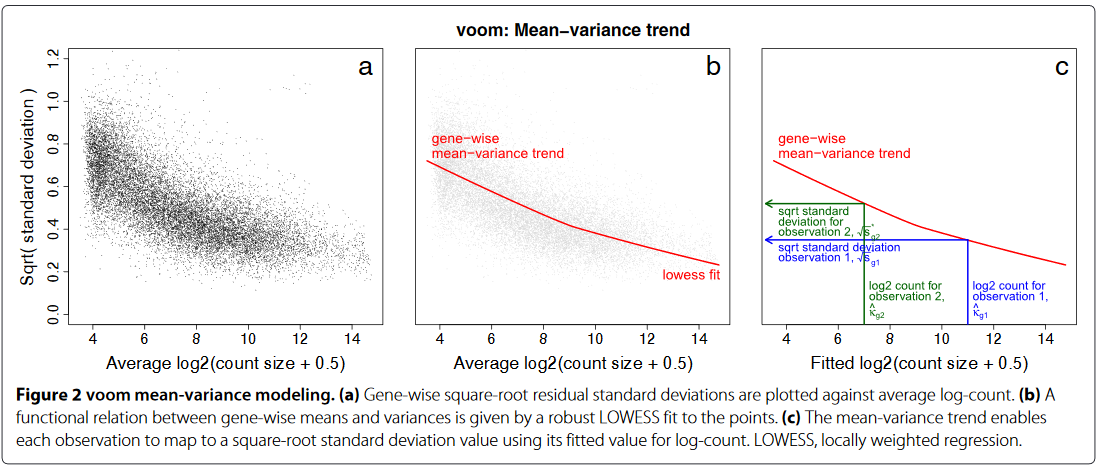
\includegraphics[width=\textwidth]{figs/voom_mean_var_trend.png}
    \label{fig:voom_mean_var_trend}
\end{figure}

This procedure accounts for the systematic relationship between the mean expression level and the residual variance.
However, this does only provide precision-weights that depend on the mean-variance trend and do not stabalize gene-wise variance estimates. 
Some genes may still have highly noisy or extreme variances due to the limited sample sizes, high biological variability or other random effects.
To solve this, the emperical Bayes method comes in.
It targets the residual variance from each gene-wise models by borrowing information across all genes to estimate the pooled prior variance, and shrinks individual gene-wise variances towards this pooled prior.
T- and F-tests can than be performed using this shrinked variance, for which we call them \textit{moderated} tests.

The main take away is that voom corrects for the systematic mean-variance trend across genes and samples, making model fitting more accurate, while eBayes stabalizes the individual gene-wise variance estimates by borrowing strength across genes, which is critical for robust hypothesis testing.
        \subsection{VoomCLR}
Next, we show how VoomCLR uses the Limma-Voom framework in order to account for compositional bias and the bias on the effect sizes.
The first thing VoomCLR does, is CLR transforming the cell counts (Formula \ref{formula:CLR}).
This is performed to deal with the composition bias.
However, compositional transformations do not stabalize the variance (it is a function of the mean).
For this reason, the transformed counts are inputed into the Limma framework to first account for the mean-variance structure using heteroscedasticity weights.
Next, the authors of the LinDA paper saw that the CLR transformation in combination with linear models result in biased effect sizes in respect to the effect sizes one would obtain based on the absolute abundances.
In order to correct for this, the mode of the effect size across cell types is used.

Next, we will explain why this is used as a correction.
If we consider a log-linear model on the absolute abundance $X_{ip}$, we get \ref{formula:loglinearXip}.
By assuming that the CLR transformed relative abundance $Y_{ip}$ can be written as the CLR transformed absolute abundance plus an estimation error $e_{ip}$, we can say that the model looks as follows (Formula \ref{formula:clr_model}).

\begin{equation}
    \log X_{ip} = C_i^T \beta_p + \epsilon_{ip}
    \label{formula:loglinearXip}
\end{equation}

\begin{align}
    \log \left\{\frac{Y_{ip}}{\left(\sum_p Y_{ip}\right)^{i/p}}\right\} &= \log X_{ip} + e_{ip} - \left\{\frac{1}{p} \sum_p \log (X_{ip} + e_{ip})\right\} \\
        &= C_i^T (\beta_p - \bar{\beta}) + (e_{ip} - \bar{\epsilon}_i)
    \label{formula:clr_model}
\end{align}

From this follows that when modeling CLR-transformed data, you are provided with estimates for $\beta_p - \bar{\beta}$, while we want estimates for $\beta_p$.
Next, an additional assumption is taken: the mode of $\beta_p$ across $p$ is zero.
Given this assumption, $\bar{\beta}$ can be estimated by shifting the histogram of our estimates of $\beta_p - \bar{\beta}$ such that it has a mode of zero.
The shift is our estimate for $\bar{\beta}$, i.e., $\hat{\bar{\beta}}$.

The now bias corrected estimates are used in the models.
The residual variance of the linear model is shrunken using Empirical Bayes and using the shrinked variance, moderated t- and F-statistics are calculated on the parameter.
The t-test tests to the null hypothesis that the coefficient is equal to zero.
The F-test tests to the null hypothesis that the model has at least one non-zero coefficient.
The F-statistic is calculated as $\frac{MSR}{MSE}$, with MSR the variation explained by the model and MSE the residual unexplained variation.

    
    \section{Causal Inference}
\subsubsection{CI vs regular regression analysis}

One major distinction that we need to make is the difference between causal inference and regression analysis.
Regression analysis statistically models the relationship between a dependent variable and a set of independent variables. 
However, this does not imply that these relationships are causal.
Furthermore, regression analysis does not take into account the direction of the relationship.
Demonstration of causality is a logical and experimental, rather than statistical, problem. 
An apparently strong relationship between variables could stem from many causes, including the influence of other currently unmeasured variables.
The causal inference methods try to balance the data in such a way that the confounders are equally distributed between the groups.
This can be done by matching, IPW, using counterfactuals...

\subsubsection{Identifiability assumptions}

One set of assumptions that is taken to identify causal effects in observed data, are the identifiability assumptions: consistency, positivity, and exchangeability.
These are important, as this enables the identification of causal effects in data that is not (perfectly) randomized. 

\begin{itemize}
    \item Exchangeability: The treatment groups need to be similar to each other in every aspect (except for the treatment). 
    In observational studies this is often relaxed to conditional exchangeability, as the groups have different characteristics by design. 
    This does mean that there should be no unmeasured confounders.
    \item Consistency: The treatment of interest should be clearly defined and applied uniformly across individuals
    \item Positivity: There should be a non-zero probability of being assigned to each treatment group for every individual given its characteristics.
\end{itemize}

\subsubsection{IPW}

Inverse Probability weighting is a method used to minimize confounding when estimating treatment effects from observational data.
By calculating a propensity score by using logistic regression on the treatment using the confounders, a weight can be derived.
This propensity score is the chance of an observation to belong to the treated class given its covariates.
In the thesis we get an ATE by calculating the weighted mean both populations (Formula \ref{formula:IPW}).

\begin{equation}
    \bar{x} = \frac{\sum_{i=1}^{n} w_i x_i}{\sum_{i=1}^{n} w_i}
    \label{formula:IPW}
\end{equation}

\subsubsection{G-computation}

G-computation is a causal inference technique that applies outcome modeling instead of treatment modeling.
In this technique, a model is fitted to the outcome variables.
In our case, this was a simple multivariate linear regression.
Next, counterfactuals are constructed.
This is the exact same dataframe twice: once with all individuals artificially put as 'diseased' and once with all individuals artificially set as 'healthy'.
The model is used to predict the outcomes of the counterfactual individuals, which are then used to get an estimate of the ATE.

\subsubsection{TMLE}

Lastly, the TMLE technique is applied, which combines treatment modeling and outcome modeling in a very clever way.
The analysis contains the following steps:

\begin{itemize}
    \item Fit an outcome model.
    \item Predict counterfactuals.
    \item Fit a treatment model.
    \item Calculate the IPW for each observation, which they call the clever covariate. 
    $H_A$ will be the corresponding IPW weight if the individual was treated or untreated.
    \item The fluctuation parameter is calculated based on the outcome model estimate (for the right treatment) and the clever covariate. 
    This is calculated using a logistic regression model using the logit transformed outcome as an offset.
    The information in the fluctuation parameter tells us how much to change or fluctuate the initial outcome estimates.
    \item The initial outcome estimates are updated using the fluctuation parameter.
    \item Calculation of the ATE using these updated outcomes for both populations.
\end{itemize}


    
    % Terms
    \newpage
    \subsection{Terms}

\begin{itemize}
    \item \textbf{Lowess fit} = Stands for \textit{\underline{LO}cally \underline{WE}ighted \underline{S}catterplot \underline{S}moothing}.
    It fits simple models localized to subsets of the data in order to build up a function that describes the deterministic part of the variation in the data, point by point.
    \item \textbf{Degrees of Freedom} = the maximum number of logically independent values, which may vary in a data sample. 
    \item \textbf{Standard deviation} = The interval of one standard deviation of the mean (on each side) in a normal distribution contains 68\% of the data. 2$\sigma$ contains 95\%, and 3$\sigma$ contains 99.7\%.
\end{itemize} 

\end{document}